\subsection{Párovacia halda} 
\paragraph{Popis.}
Párovacia halda je ďalším druhom samoupravujúcej sa haldy. Opäť sa budeme pozerať na amortizovanú časovú zložitosť jej operácií.
Je to všeobecná halda, teda počet synov nie je obmedzený.

Základná procedúra, ktorú budeme pri popise párovacej haldy používať je spájanie (\emph{linking}) dvoch háld,
pričom sa halda s väčším kľúčom v koreni napojí pod tú s menším kľúčom.
V našej implementácií sa nový vrchol napája vždy ako prvý syn.

\paragraph{Operácie.}
Operácia $\meld(i,j)$ jednoducho spojí ("zlinkuje") dané dve haldy. $\mathop{\mathit{Insert}}(x)$ podobne len prilinkuje
novú jednoprvkovú haldu.
Operácia $\dec(v, \Delta)$ najprv zníži hodnotu vrcholu $v$, a keďže môže byť porušená podmienka pre haldu,
strom zakorenený vo vrchole $v$ sa odtrhne a prilinkuje ku zvyšku. Časové zložitosti pre všetky tieto operácie
sú $O(1)$. Najzaujímavejšie na párovacích haldách je $\delmin$. Po odstránení koreňa ostane les jeho detí.
Môžeme zvoliť niekoľko prístupov ako z detí opäť vytvoríme jeden nový strom.

%Naivné riešenie hovorí, že si vyberieme jedno dieťa a ostatné k nemu prilinkujeme. Už na prvý pohľad vidíme,
%že pri nesprávnom zvolení prvého dieťaťa môže byť časová zložitosť takéhoto algoritmu $\Omega(n)$.

%Ďalší, o niečo lepší nápad je deti najprv popárovať a potom prilinkovať. S výhliadkami do budúcnosti nám tento algoritmus dá 
%amortizovanú časovú zložitosť $O(\sqrt{n})$.

%Prečo dieťa s najmenším kľúčom? V tom článku je len taký konkrétny príklad na obrázku, ale pod tým je, že pri naive sa vyberá %hociktoré dieťa
%Naivné riešenie hovorí, že si vyberieme strom s najmenším koreňom a ostatné k nemu prilinkujeme.
\paragraph{Operácia $\delmin$ a časová zložitosť.}
Naivné riešenie hovorí, že si vyberieme jedno dieťa a ostatné k nemu prilinkujeme.
Takéto riešenie má v najhoršom prípade až lineárnu zložitosť (existuje postupnosť $n$ operácií,
ktorá bude trvať $\Omega(n^2)$).

O niečo lepší nápad je deti najskôr v prvom prechode zlinkovať po pároch
a v druhom prechode prilinkovať zvyšné stromy s jedným vybratým.
Takýto algoritmus už garantuje amortizovanú časovú zložitosť $O(\sqrt{n})$
(a existuje postupnosť $n$ operácií, ktorá trvá $\Omega(n\sqrt{n})$).

\begin{figure*}
\centering
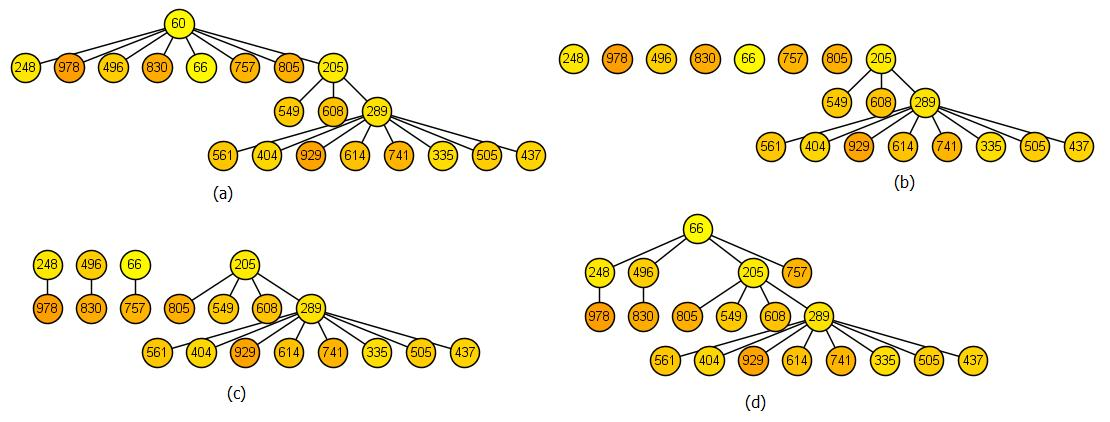
\includegraphics[width=2\columnwidth]{obrazky/pairdel.png}
\caption{\emph{Vymazanie minima z párovacej haldy.} 
(a)~pôvodná halda, (b)~halda po odstránení minima, t.j.\ koreňa stromu; (c)~situácia po prvom
prechode, keď zlinkujeme dvojice stromov zľava doprava, (d)~halda po spájaní: v druhom
prechode postupujeme sprava doľava a postupne linkujeme zvyšné stromy od najpravejšieho koreňa k najľavejšiemu.} 
\label{img:pairdel} 
\end{figure*}

Keď si dáme väčší pozor na to, ako deti párujeme, môžeme dosiahnnuť ešte lepšie 
výsledky. \citet{pairing} dokázali, že ak v prvom prechode párujeme synov v poradí,
v akom boli prilinkovaní od najmladšieho a v druhom prechode ich linkujeme sprava doľava,
operácie $\ins$, $\meld$, $\dec$ a $\delmin$ majú amortizovanú zložitosť $O(\log n)$.
Skutočná časová zložitosť týchto operácií je dodnes otvorený problém. 
%\citet{pettie} dokázal, že $\ins$, $\meld$ a $\dec$ majú v skutočnosti lepšiu ako logaritmickú zložitosť
%($O(2^{2\sqrt{\log\log n}})$).
Experimentálne výsledky \citep{moret91,pettie02} však dokazujú, že párovacia halda
je v praxi veľmi efektívna dátová štruktúra.

\citet{pairing} navrhli niekoľko variant párovacej haldy. Jedna alternatíva je pri odstraňovaní minima
postupne párovať zvyšné stromy (na viacero prechodov), až kým nám neostane jediný strom.
Tieto ďalšie riešenia sme zatiaľ nevizualizovali, ale plánujeme ich implementovať počas budúcej práce na projekte.

% Ostatné riešenia sme zatiaľ neimplementovali, preto len spomenieme, že sú popísané napríklad v \cite{pairing}.

% Aby boli ale operácie efektívne, musíme zvoliť správnu reprezentáciu tejto dátovej štruktúry. V našom programe sme použili 
% reprezentáciu pomocou binárneho stromu (\emph{binary tree represetation}), ktorú naprogramoval Viktor Tomkovič. V každom vrchole sa uchováva ľavý smerník na prvého syna, pravý smerník na nasledujúceho brata a ešte jeden smerník na rodiča.

% \paragraph{Vizualizácia.}
% Pri implementácií sme si pomohli nasledujúcim trikom: Pri odstránení minima koreň haldy ostáva jej súčasťou
% až do konca operácie, ale je zneviditeľnený. Navonok teda vyzerá, že po odstránení minima ostal les synov,
% v skutočnosti však máme stále jednu haldu. Takto využijeme už naprogramované rozloženie vrcholov
% a nemusíme zvlášť doprogramovať algoritmus pre rozloženie lesu.


